% ====================================================================
%   그리기 패키지  --> 모두 뺴기.
% 
%  이 패키지는 Cation에 footnote를 추가하면 footnote 내용이 보이지 않음
%  원인은 잘 모르지만, 회로 그림은 별도로 그려서(pdf 로 만들어서 ) 사용을 해야 할 것 같음.
%
% \usepackage[siunitx, RPvoltages]{circuitikz}  % 회로부품 그리기.
%%
%%  TikZ -  초기 선언문 
%\usepackage{tikz} 
%\usepackage{pgfplotstable}
%\usepackage{pgfplots}
%\usetikzlibrary{arrows,patterns}
%\usetikzlibrary{decorations.markings}
%
%   모든 그림(tikz, circuit)은 pdf 로 불러오기.  2021.09.03.
%
% ====================================================================

\documentclass[a4paper]{book} 

\usepackage[hangul]{kotex}  % 좀 더 다양한 한글 표현이 가능
\usepackage{adjustbox} %this
%\usepackage{kotex}  
\usepackage{graphicx}
\usepackage{amsmath}
\usepackage[framemethod=TikZ]{mdframed}
\usepackage{amsthm}
\usepackage{amssymb} % 수학의 그러므로를 표현하기 위함 
\usepackage{ulem} % 글자 취소선 넣기  \sout{  ... }
\usepackage[]{mcode} % MATLAB code 넣기. mcode.sty 다운 받기 https://strikers01.tistory.com/329
%\usepackage[]{mypaper}

\usepackage{listings}  % 출처 :  https://frombc7197.tistory.com/5224
\lstset{numbers = left, numbersep=8pt, breaklines=true} % CODE에 줄번호 넣고 싶을 떄...

\usepackage[most]{tcolorbox}

% 색상의 채워진 삼각형을 그리기 위함.
\usepackage{etoolbox}
\usepackage{tikz}
%\newrobustcmd*{\square}[1]{\tikz{\filldraw[draw=#1,fill=#1] (0,0) rectangle (0.2cm,0.2cm);}}
\newrobustcmd*{\mycircle}[1]{\tikz{\filldraw[draw=#1,fill=#1] (0,0) circle [radius=0.1cm];}}
\newrobustcmd*{\mytriangle}[1]{\tikz{\filldraw[draw=#1,fill=#1] (0,0) -- (0.2cm,0) -- (0.1cm,0.2cm);}}
% [ex]
%   a circle \mycircle{green} and a triangle \mytriangle{blue}
 % ==================================

%%%%%%%%%%%%%%%%%%%%%%%%%%%%%%
%  출처 : https://texblog.org/2015/09/30/fancy-boxes-for-theorem-lemma-and-proof-with-mdframed/
%%%%%%%%%%%%%%%%%%%%%%%%%%%%%%
%DIFINITION
\newcounter{defi}[section] \setcounter{defi}{0}
\renewcommand{\thedefi}{\arabic{section}.\arabic{defi}}
\newenvironment{defi}[2][]{%
\refstepcounter{defi}%
\ifstrempty{#1}%
{\mdfsetup{%
frametitle={%
\tikz[baseline=(current bounding box.east),outer sep=0pt]
\node[anchor=east,rectangle,fill=blue!20]
{\strut DEFINITION~\thedefi};}}
}%
{\mdfsetup{%
frametitle={%
\tikz[baseline=(current bounding box.east),outer sep=0pt]
\node[anchor=east,rectangle,fill=blue!20]
{\strut DEFINITION~\thedefi:~#1};}}%
}%
\mdfsetup{innertopmargin=10pt,linecolor=blue!20,%
linewidth=2pt,topline=true,%
frametitleaboveskip=\dimexpr-\ht\strutbox\relax
}
\begin{mdframed}[]\relax%
\label{#2}}{\end{mdframed}}
%%%%%%%%%%%%%%%%%%%%%%%%%%%%%%
%Theorem
\newcounter{theo}[section] \setcounter{theo}{0}
\renewcommand{\thetheo}{\arabic{section}.\arabic{theo}}
\newenvironment{theo}[2][]{%
\refstepcounter{theo}%
\ifstrempty{#1}%
{\mdfsetup{%
frametitle={%
\tikz[baseline=(current bounding box.east),outer sep=0pt]
\node[anchor=east,rectangle,fill=blue!20]
{\strut Theorem~\thetheo};}}
}%
{\mdfsetup{%
frametitle={%
\tikz[baseline=(current bounding box.east),outer sep=0pt]
\node[anchor=east,rectangle,fill=blue!20]
{\strut Theorem~\thetheo:~#1};}}%
}%
\mdfsetup{innertopmargin=10pt,linecolor=blue!20,%
linewidth=2pt,topline=true,%
frametitleaboveskip=\dimexpr-\ht\strutbox\relax
}
\begin{mdframed}[]\relax%
\label{#2}}{\end{mdframed}}
%%%%%%%%%%%%%%%%%%%%%%%%%%%%%%
%Lemma
\newcounter{lem}[section] \setcounter{lem}{0}
\renewcommand{\thelem}{\arabic{section}.\arabic{lem}}
\newenvironment{lem}[2][]{%
\refstepcounter{lem}%
\ifstrempty{#1}%
{\mdfsetup{%
frametitle={%
\tikz[baseline=(current bounding box.east),outer sep=0pt]
\node[anchor=east,rectangle,fill=green!20]
{\strut Lemma~\thelem};}}
}%
{\mdfsetup{%
frametitle={%
\tikz[baseline=(current bounding box.east),outer sep=0pt]
\node[anchor=east,rectangle,fill=green!20]
{\strut Lemma~\thelem:~#1};}}%
}%
\mdfsetup{innertopmargin=10pt,linecolor=green!20,%
linewidth=2pt,topline=true,%
frametitleaboveskip=\dimexpr-\ht\strutbox\relax
}
\begin{mdframed}[]\relax%
\label{#2}}{\end{mdframed}}
%%%%%%%%%%%%%%%%%%%%%%%%%%%%%%
%Proof
\newcounter{prf}[section]\setcounter{prf}{0}
\renewcommand{\theprf}{\arabic{section}.\arabic{prf}}
\newenvironment{prf}[2][]{%
\refstepcounter{prf}%
\ifstrempty{#1}%
{\mdfsetup{%
frametitle={%
\tikz[baseline=(current bounding box.east),outer sep=0pt]
\node[anchor=east,rectangle,fill=red!20]
{\strut Proof~\theprf};}}
}%
{\mdfsetup{%
frametitle={%
\tikz[baseline=(current bounding box.east),outer sep=0pt]
\node[anchor=east,rectangle,fill=red!20]
{\strut Proof~\theprf:~#1};}}%
}%
\mdfsetup{innertopmargin=10pt,linecolor=red!20,%
linewidth=2pt,topline=true,%
frametitleaboveskip=\dimexpr-\ht\strutbox\relax
}
\begin{mdframed}[]\relax%
\label{#2}}{\qed\end{mdframed}}
%%%%%%%%%%%%%%%%%%%%%%%%%%%%%%

\usepackage{nameref}   % reference 이름으로 링크를 걸고 싶은 경우.
% 목차 또는 ref 에 마우스 클릭시 페이지 이동하는 부분.
\usepackage{hyperref}
\hypersetup{
    colorlinks=true,
    linkcolor=blue, % 연결 문구의 색상을 정의 한다.
    citecolor=black,
    filecolor=black,
    urlcolor=black,
}

\usepackage{amsfonts}  % https://www.physicsread.com/latex-mathbb/
\usepackage{caption}
\usepackage{subcaption}
\usepackage{color} % 글자 색상을 바꾸는 패키지. \textcolor
%\usepackage{verbatim}  % 문서내 코드 넣기 - https://ka373.tistory.com/41


\usepackage{multirow}	% 셀 병합을 위하여 사용하는 패키지. (https://tablesgenerator.com)
\usepackage{ftnxtra}  % caption 에 footnote 넣기 위한 패키지. https://tex.stackexchange.com/questions/10181/using-footnote-in-a-figures-caption
\usepackage{fnpos} % \makeFNbelow by default 

% 그림 배치를 왼쪽/중간/오른쪽 글씨 겹침에 사용함
% 출처 : http://www.ktug.org/xe/index.php?document_srl=243219&mid=KTUG_open_board
\usepackage{wrapfig}

\usepackage[onehalfspacing]{setspace}  % singlespacing, onehalfspacing, doublespacing 
\usepackage[left=2.5cm,right=4.5cm,top=5cm,bottom=4cm,a4paper]{geometry}

% 패키지의 위치에 따라 에러가 날수도 안날수도 있음.

%\usepackage[table,xcdraw]{xcolor} % 표(table)의 배경색을 넣기 위함.
%\usepackage{alertmessage}% ==========
%  \alertinfo{}
%  \alertsuccess{}
% \alertwarning{}
% \alerterror{}
 % ==================================




\usepackage{makeidx}  % index 전처리.
\makeindex

% Header and Footer Stuff
% https://ko.overleaf.com/learn/latex/Headers_and_footers
\usepackage{fancyhdr}
\pagestyle{fancy}
\fancyhead{}
\fancyfoot{}
%\fancyfoot[R]{\thepage}
\fancyhead[LE,RO]{\thepage}
\fancyhead[RE,LO]{\leftmark}
\renewcommand{\headrulewidth}{2pt}
\renewcommand{\footrulewidth}{1pt}

% ====================================================================
% ====================================================================

\author{여동훈  } 
\title{ 공돌이의 수학정리노트} 

\begin{document} 

%	\maketitle

%	\tableofcontents  
%	\listoffigures
%	\listoftables

	[Youtub] https://www.youtube.com/watch?v=Z9dvM7qgN9s\&t=446s


[출처] /Users/leejaekun/.gitconfig
1.VS Code를 Git diff tool

1. 명령어중에 code --help를 실행하면 도움말이 표시되는지 확인 합니다.\\
표시되지 않는다면 \\
macOS: Command Palette에서 Shell Command: Install ‘Code’ command in path를 선택합니다.\\
윈도우즈: VS Code 를 설치하는 동안 PATH 에 추가하기를 선택합니다.\\
리눅스: .deb 또는 .rpm 패키지를 사용하여 설치합니다.\\

\noindent > git config --global core.editor "code --wait"\\
에디터를 visual studio code 로 설정하고, code를 닫기 전까지 응답하지 않음. \\

\noindent > git config --global core.autocrlf true  (window user 의 경우 )\\
\noindent > git config --global core.autocrlf input (mac user 의 경우 )\\
%
\begin{figure} [!htbp] % [!htbp] 
	\centering
	\captionsetup{justification=centering,margin=1cm}
	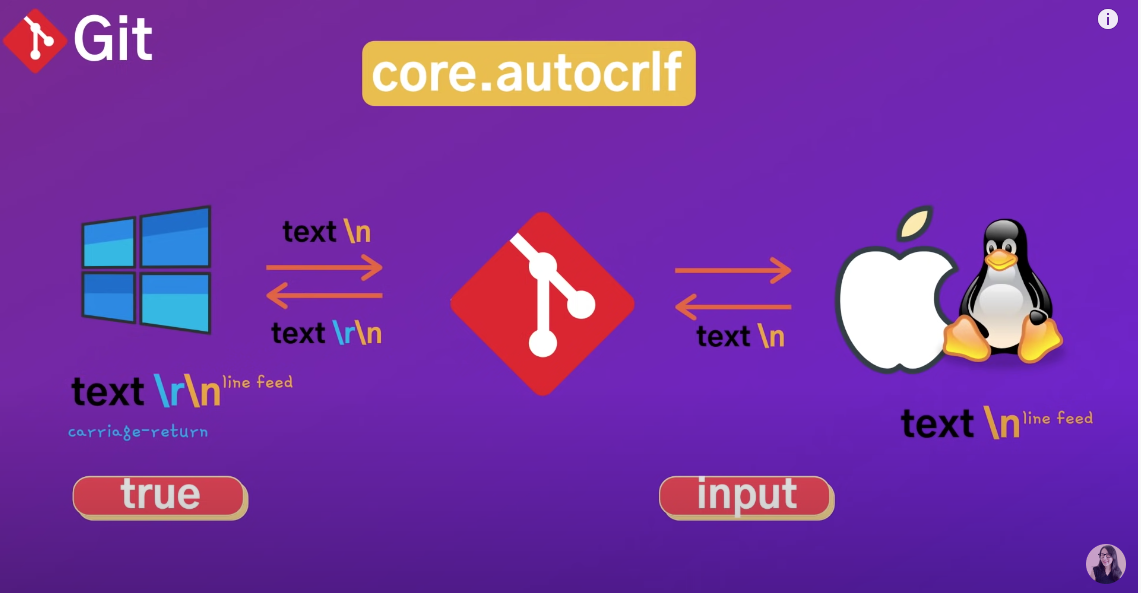
\includegraphics[width=0.7\linewidth]{./fig/autocrlf.png}
	\caption{window / max의 캐리지리턴}
	\label{fig:autocrlf}
\end{figure} 
%




\newpage
\setstretch{1.6} 
\noindent [출처] \href{https://reddb.tistory.com/146?category=948284}{\color{blue}{https://reddb.tistory.com/146?category=948284}}

\noindent \textbf{git init} : 초기화. .git 폴더가 만들어 진다.\\
%
\textbf{git status} : git 의 상태를 출력 합니다.\\
%
\begin{itemize}
	\item On branch master : 현재 마스터 브랜치가 존재
	\item No commits yet : 아직 커밋한 파일이 없음 
	\item nothing to commit : 현재 커밋할 파일이 없음.
\end{itemize}
%
\begin{figure} [!htbp] % [!htbp] 
	\centering
	\captionsetup{justification=centering,margin=1cm}
	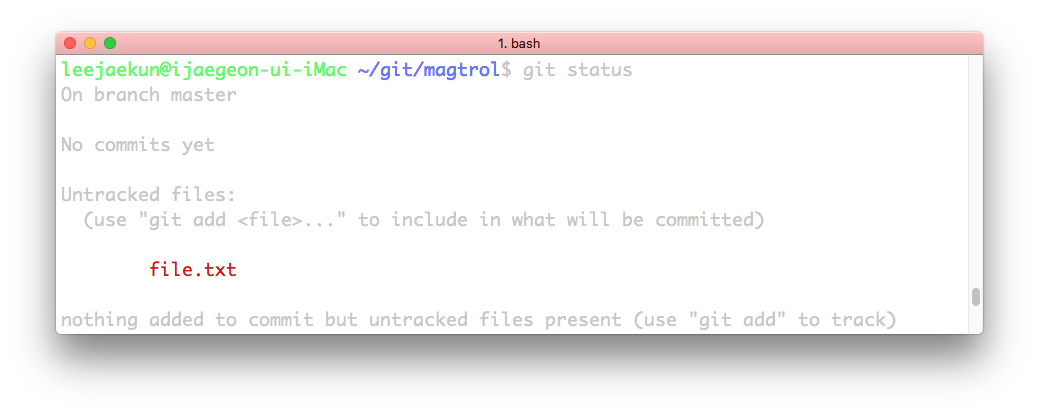
\includegraphics[width=0.7\linewidth]{./fig/status.png}
	\caption{git status 예제}
	\label{fig:status}
\end{figure} 
%
파일을 생성을 하고 git status를 입력을 하면 Untracked files 하는 변화된 내용이 출력됩니다.
깃에서 버젼관리를 하지 않는 파일들을 Untracked files 라고 합니다.\\
%
\textbf{git add} : 파일을 스테이지로 올립니다.
%
\begin{figure} [!htbp] % [!htbp] 
	\centering
	\captionsetup{justification=centering,margin=1cm}
	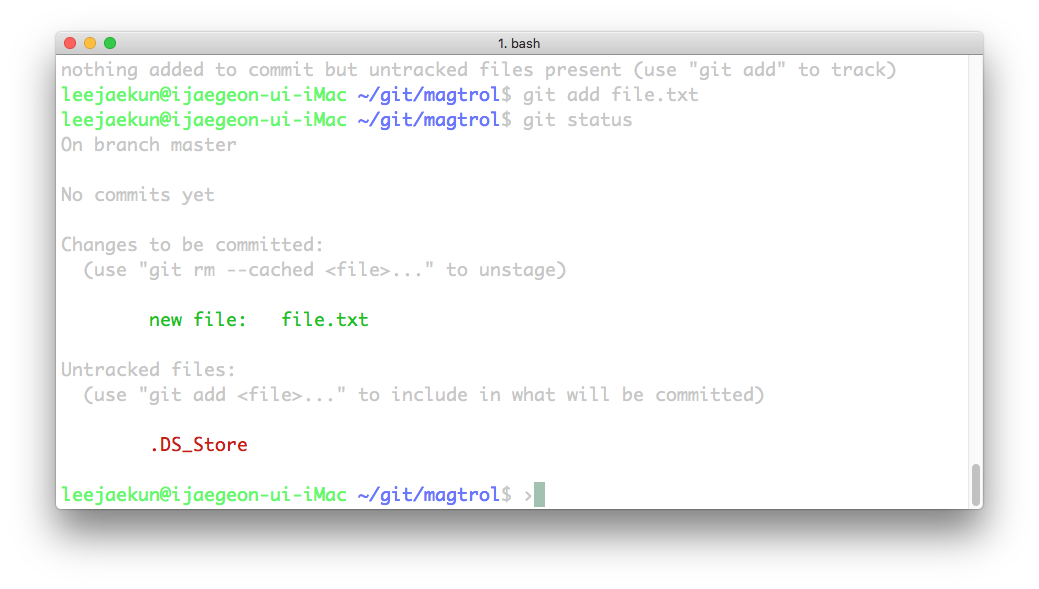
\includegraphics[width=0.7\linewidth]{./fig/add.png}
	\caption{git add 예제}
	\label{fig:add}
\end{figure} 
%
git status 를 입력하면 Change to be commited 라는 변화된 내용으로 출력 됩니다.
이는 파일이 커밋할 준비가 되었다는 상태입니다. \\
%
\noindent \textbf{git commit} : 파일을 커밋합니다. \\
그림\ref{fig:commit}\과 같이 git commit -m "넣고 싶은 메시지" 형태로 입력을 합니다. \\
%
\begin{figure} [!htbp] % [!htbp] 
	\centering
	\captionsetup{justification=centering,margin=1cm}
	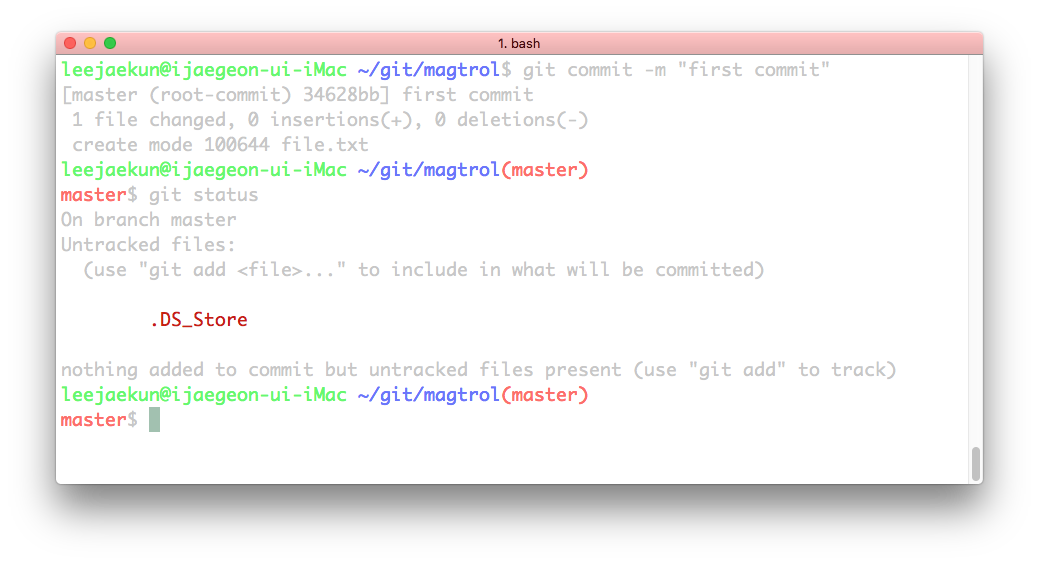
\includegraphics[width=0.7\linewidth]{./fig/commit.png}
	\caption{git commit 예제}
	\label{fig:commit}
\end{figure} 
%
 \textbf{git log} : commit 되어 있는 상태를 보여준다. \\
 내가 입력한 메시지(수정내용 요약) 내용을 포함한다. \\
 %
\begin{figure} [!htbp] % [!htbp] 
	\centering
	\captionsetup{justification=centering,margin=1cm}
	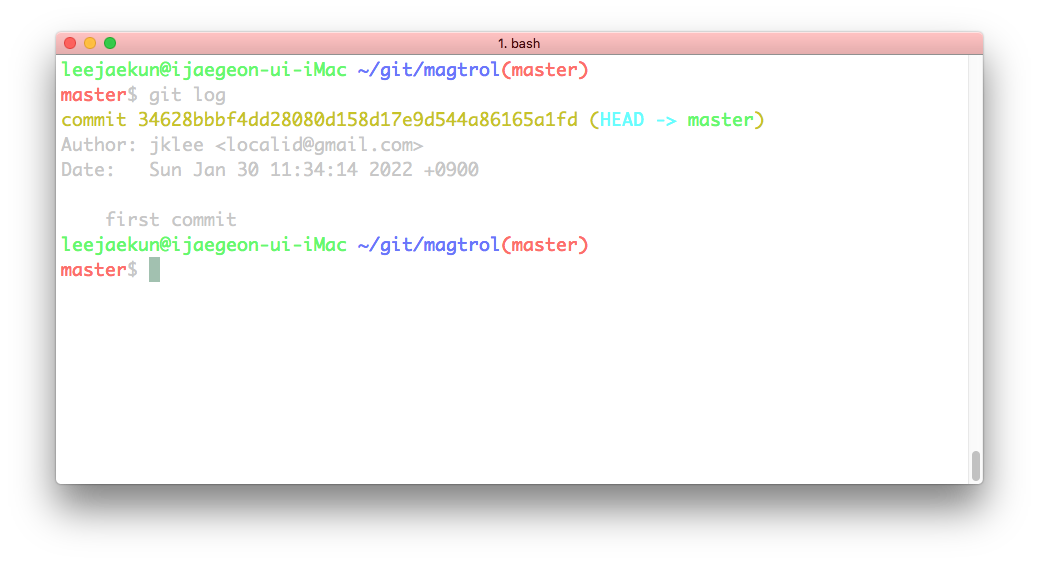
\includegraphics[width=0.7\linewidth]{./fig/log.png}
	\caption{git log 예제}
	\label{fig:log}
\end{figure} 
%
 
 \newpage
 \noindent \large{\href{https://gist.github.com/480/4681b67d2a906db8c6c1321cc678f05f}{\textbf{\color{blue}깃 리모트 변경 하기}} }\\
\newline \normalsize
% 
\textbf{기존 리포지토리 깔끔하게 pull / push} \\
git pull \\
git add . \\
git commit -m "clean push" \\
git push \\
%
\newline
\textbf{기존 리포지토리 remote 제거} \\
git remote remove origin \\
%
\newline
\textbf{새 리포지토리 remote 추가} \\
git remote add origin https://github.com/계정/리포지토리 \\

 \newpage
 \noindent \href{https://www.yalco.kr/lectures/git-github/}\textbf{\color{blue}{얄코 강좌}} \\
 iTerms2 설치와 터미널 셋팅 \\
 %
\begin{figure} [!htbp] % [!htbp] 
	\centering
	\captionsetup{justification=centering,margin=0.5cm}
	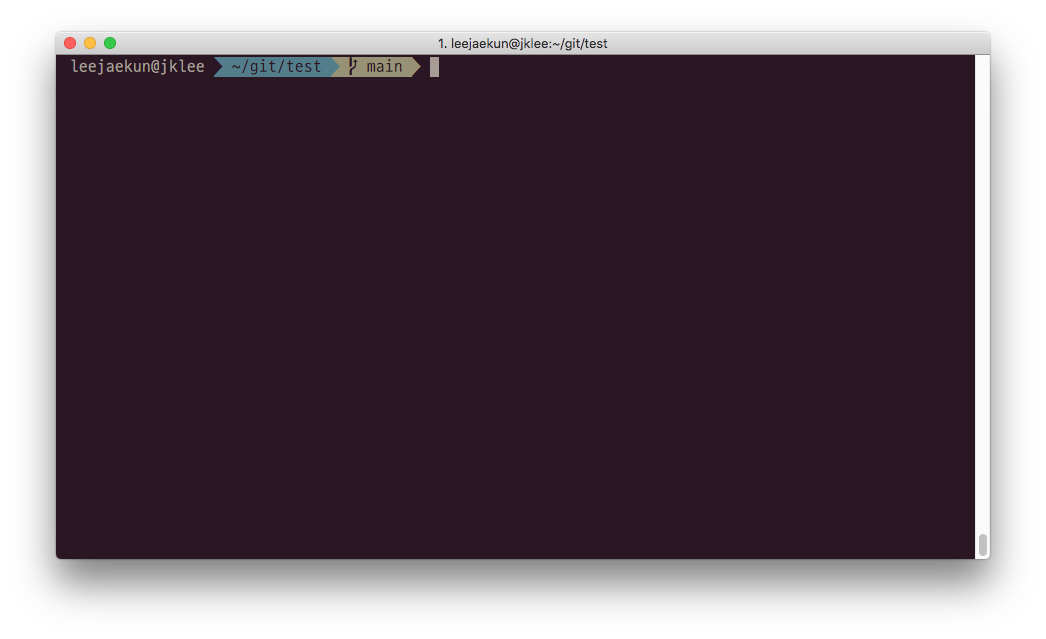
\includegraphics[width=0.7\linewidth]{./fig/zsh-iTerms2.png}
	\caption{zsh 설치 후, iTerms2 화면 예제}
	\label{fig:iTerms2}
\end{figure} 
%
$\rhd$  git remote add origin https://github.com/leejaekun/GitMemo.git \\
$\rhd$ git branch -M main \\
$\rhd$  git push -u origin main \\
Username for 'https://github.com': leejaekun\\
Password for 'https://leejaekun@github.com':\\
오브젝트 나열하는 중: 20, 완료.\\
오브젝트 개수 세는 중: 100\% (20/20), 완료.\\
Delta compression using up to 4 threads\\
오브젝트 압축하는 중: 100\% (19/19), 완료.\\
오브젝트 쓰는 중: 100\% (20/20), 2.90 MiB | 1.15 MiB/s, 완료.\\
Total 20 (delta 2), reused 0 (delta 0), pack-reused 0\\
remote: Resolving deltas: 100\% (2/2), done.\\
To https://github.com/leejaekun/GitMemo.git\\
 * [new branch]      main $->$ main\\
branch 'main' set up to track 'origin/main'.\\
\\



 
 
 


%  	 \input{phasor.tex}
%  	\input{impulse.tex}

	\printindex
\end{document} 